\documentclass[12pt, notitlepage]{article}

\usepackage{fullpage}
\usepackage{listings}
\usepackage{color}
\usepackage{graphicx}
\usepackage{caption}
\usepackage{subcaption}
\usepackage{url}

\definecolor{gray}{rgb}{0.5,0.5,0.5}
\definecolor{dkgreen}{rgb}{0,0.6,0}
\definecolor{mauve}{rgb}{0.58,0,0.82}

\usepackage{caption}
\DeclareCaptionFont{white}{\color{white}}
\DeclareCaptionFormat{listing}{\colorbox{gray}{\parbox{\textwidth}{#1#2#3}}}
\captionsetup[lstlisting]{format=listing,labelfont=white,textfont=white}

\lstset{
%backgroundcolor=\color{white},
%frame=single,
%title=\lstname, 
keywordstyle=\color{blue}, 
commentstyle=\color{dkgreen}, 
stringstyle=\color{mauve},
showspaces=false,               
showstringspaces=false
}

\begin{document}



\title{Habitat Simulation}
\author{Abel Souza, Derek Weitzel, Douglas Silva}
\date{December 7, 2012}

\maketitle

\section{Introduction}

A significant problem in wildlife management is identifying ��good�� habitat for species within the short time frames demanded by policy makers. Statistical models of the response of species presence/absence to predictor variables are one solution, widely known as habitat modeling.

The current model, called Habitat, was made by Andrew J. Tyre and is basically modeling a big landscape and filling it with creatures/animals. The landscape can be seen as a big matrix and each of its position is a cell. In those cells the algorithm fills with creatures/Individuals that will do some calculations inside it to major if this cell has a good or bad quality.

The spread out of Individuals in the landscape can be seen on the picture below in Figure \ref{fig:agentmovement}. The algorithm will determine the cell using one specific function and depending on the input that is given.


\begin{figure}[ht!]
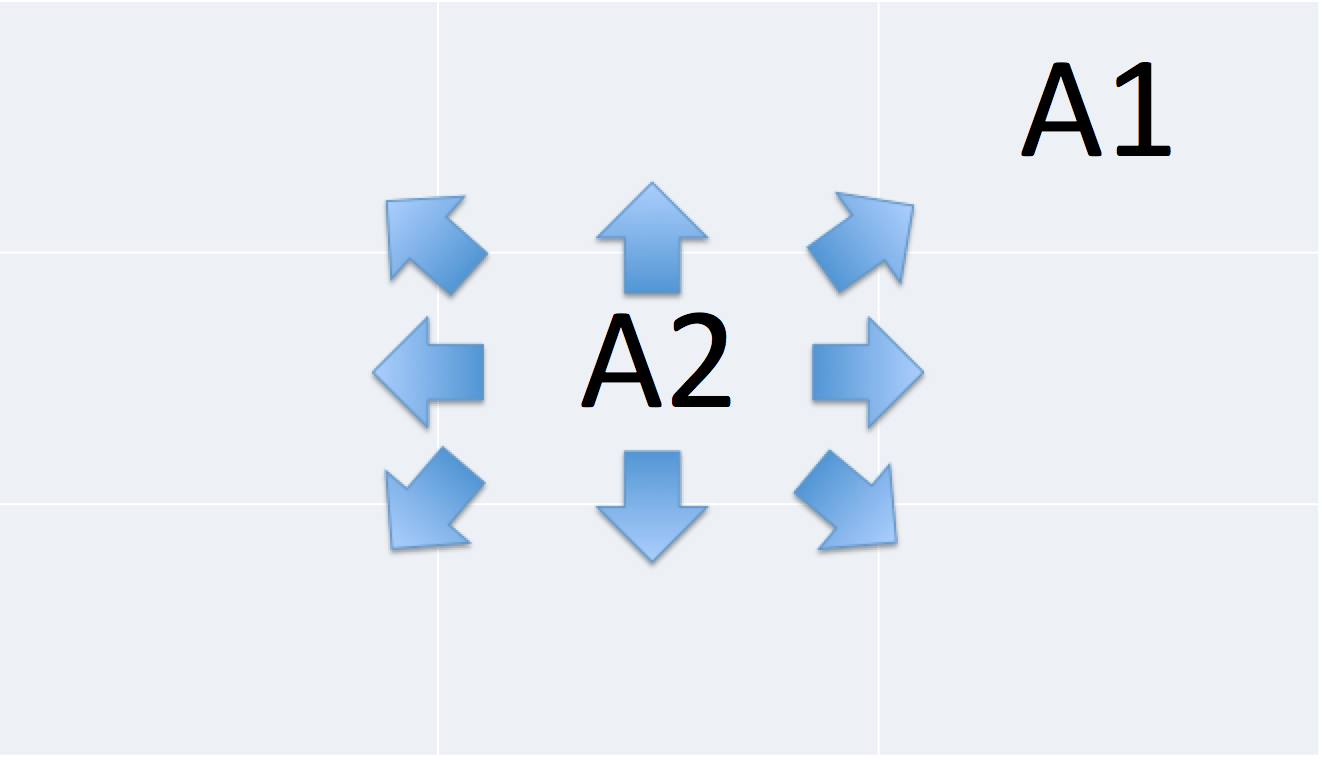
\includegraphics[width=\textwidth]{Include/agentmovement.png}
\caption{How an individual settles in one cell} \label{fig:agentmovement}
\end{figure}


One could imagine that the parallelization of this algorithm could be easy. All we basically need is to parallelize the function that spreads the Individuals out. However, there are some constraints we have to respect in order to generate the right output. These are:

\begin{itemize}
\item In each cell we can have just one Individual.
\item One Individual cannot be in two cells at the same time.
\item We cannot change the structure of the code, because the author is always changing it.
\end{itemize}

\section{Implementation}

We started our efforts of parallelizing the application by analyzing it by using the Google Profiler tool. The result of the profile, as can be seen in the Figure \ref{fig:originalcall}, showed us that about 58\% of the application running time was being spent inside the disperse4() function.

\begin{figure}[ht]
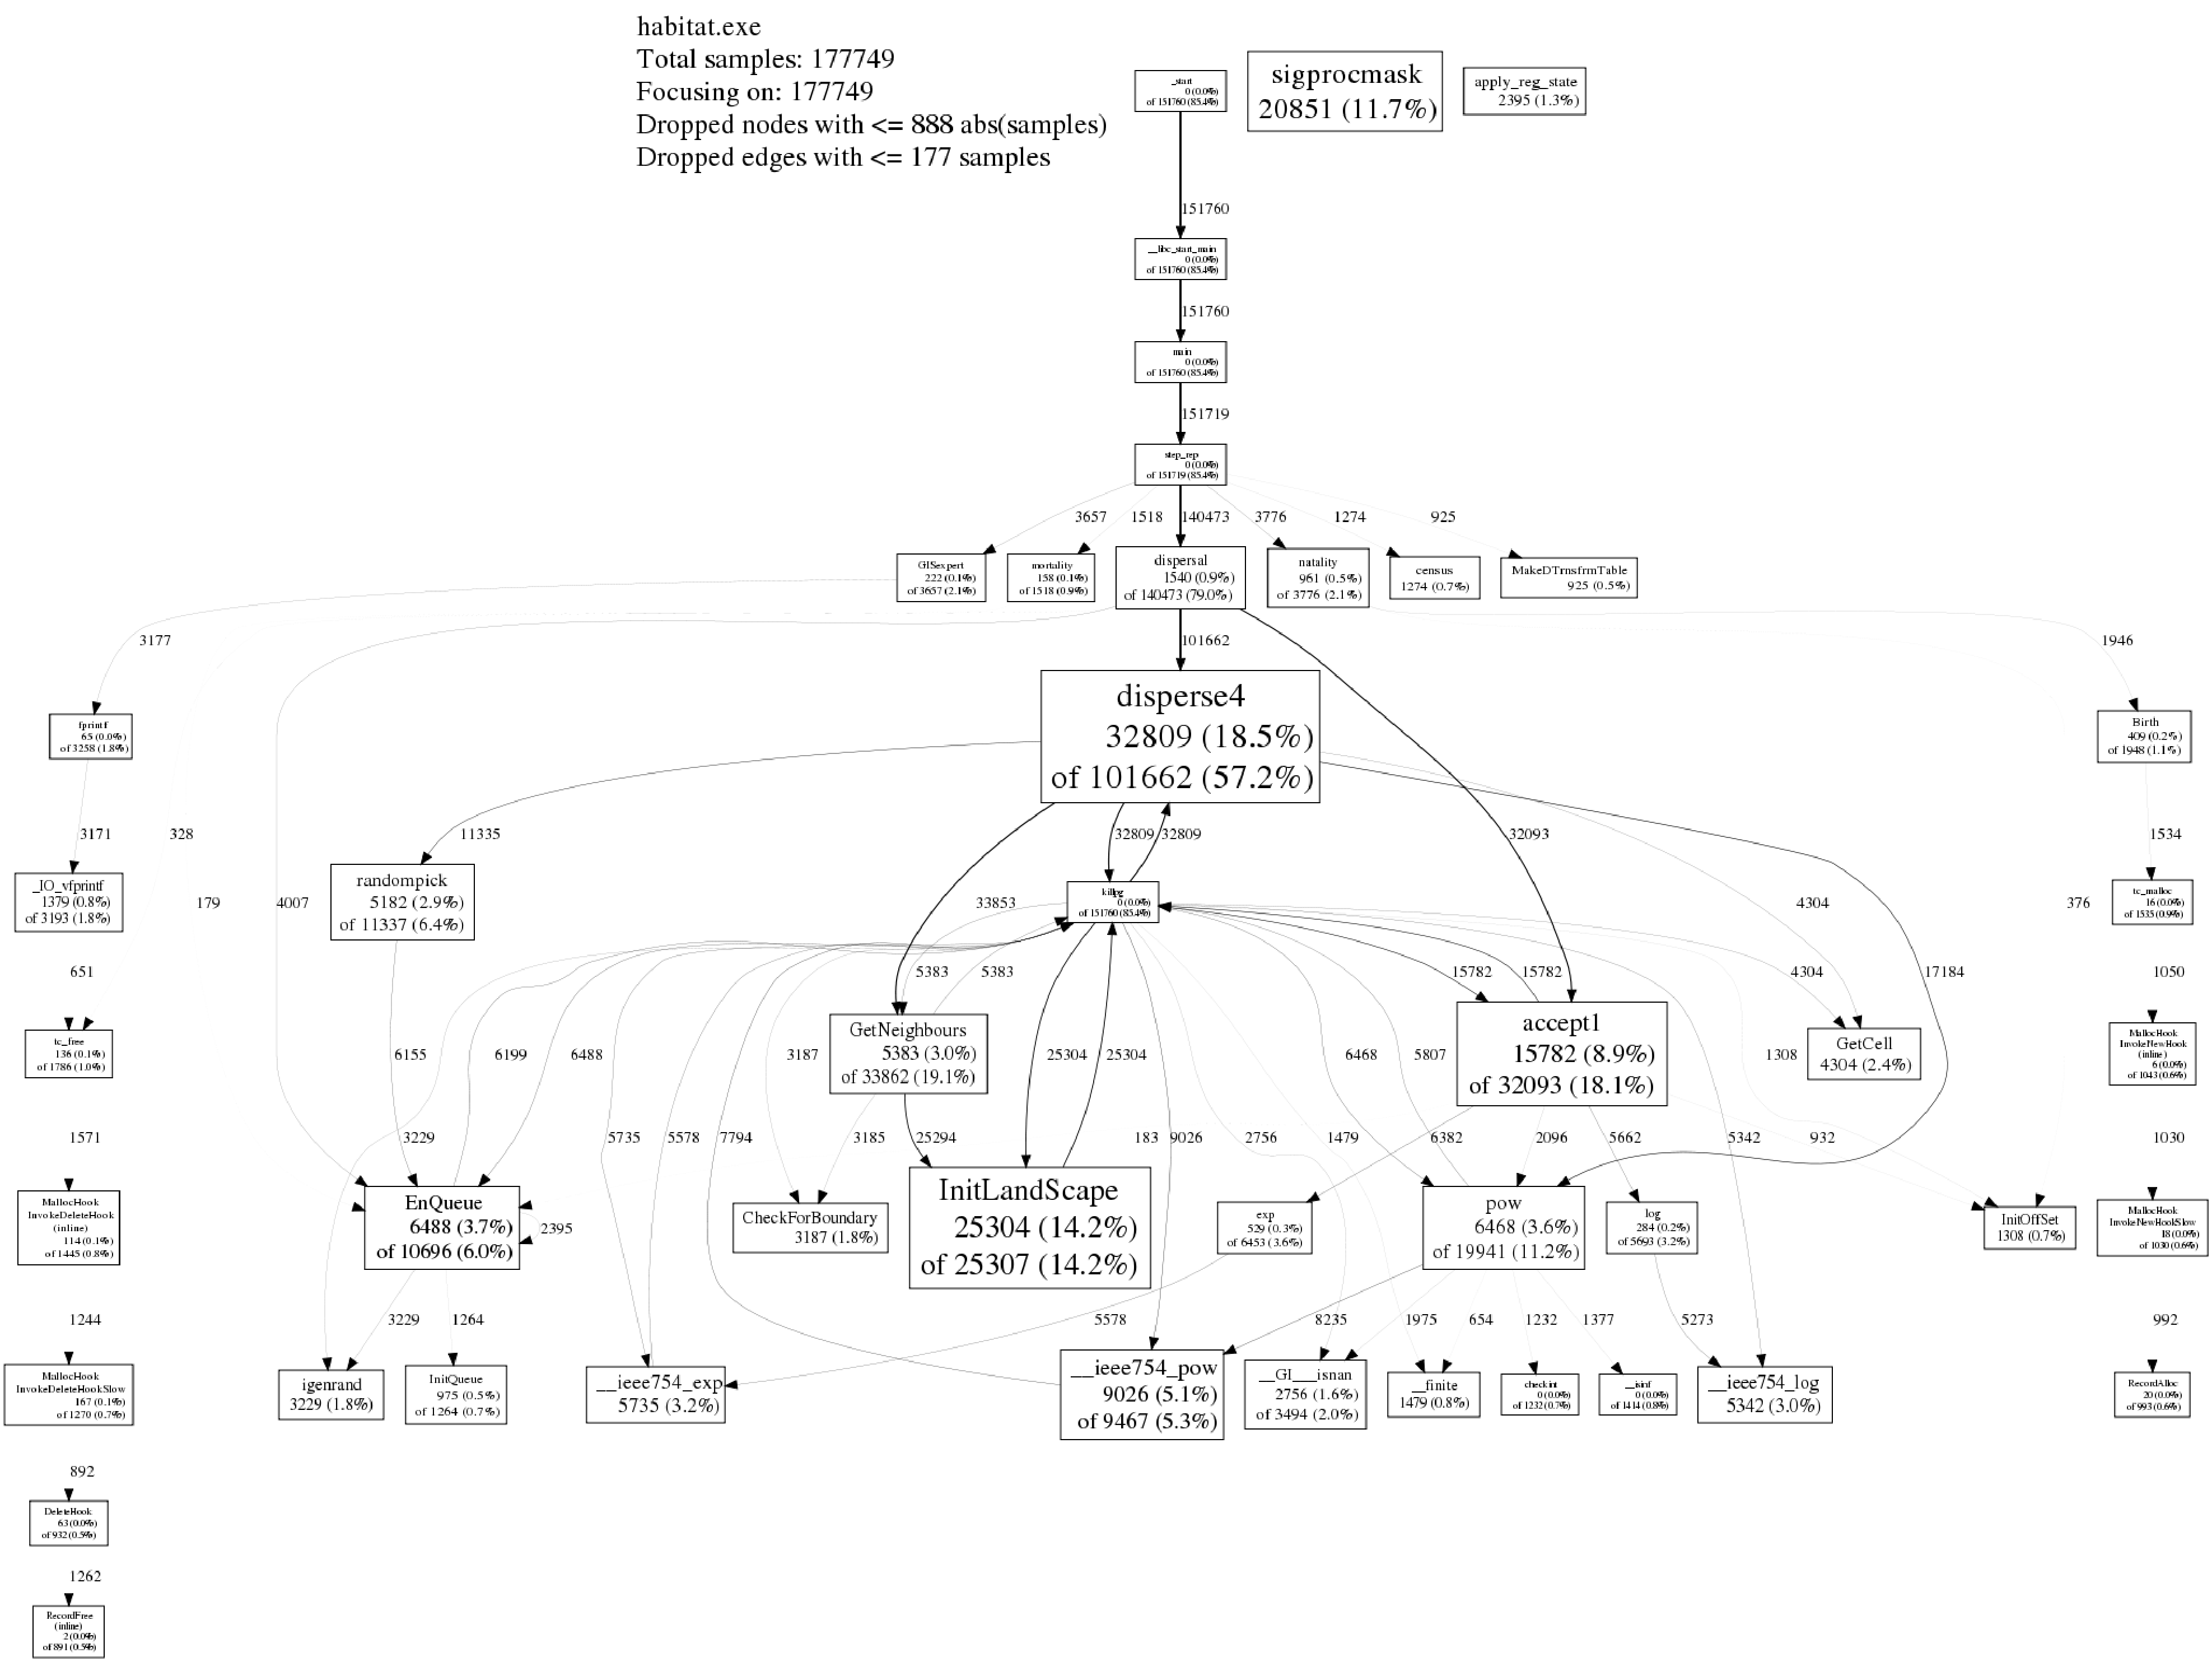
\includegraphics[width=\textwidth]{Include/originalcall.pdf}
\caption{Call graph for the non-parallelized habitat simulation} \label{fig:originalcall}
\end{figure}

The disperse4() couldn�t be parallelized, because there was not any loop that would be run for a significant time, so we started by analyzing where this function was called. We found that it is just called in another single function, the disperse().

The disperse() function has a loop that will iterate through all individuals that are not settled in a position, until they find the best possible location. The individual also have a chance of dying in the journey, that is being considered inside this function.

This function takes approximately 80\% of the running time. We concluded that the best approach to parallelize the application was to use OpenMP, because this way would require a smaller amount of changes in the original source code and since only 80\% of the application could exploit parallelism, using a massive amount of threads through OpenMPI or CUDA would not really show a great improvement when compared to using a smaller quantity of threads that a single computer could provide, as can be deducted by Amdahl's law.

We also found that there was not any other section of the application that would obtain a considered advantage by being parallelized, therefore we started by modifying the code so that the loop present in the disperse() function could be run in parallel. This required that multiples lock were added through the application to avoid any data hazard. These locks were added in such manner  just one thread can work with a single cell or individual  at a single time.

Some other chances related to memory allocation were necessary to be made in the source code, to avoid some segmentation errors that we started getting when running the application in multiple cores.

These changes allowed a utilization of almost 100\% in all processors during all the application running time. We profiled the application with our changes, and we found that these modifications dramatically changed the profiler graph, as can be seen in the original call graph in Figure \ref{fig:originalcall} and compared to the parallel call graph in Figure \ref{fig:parallelcall}.

\begin{figure}[ht]
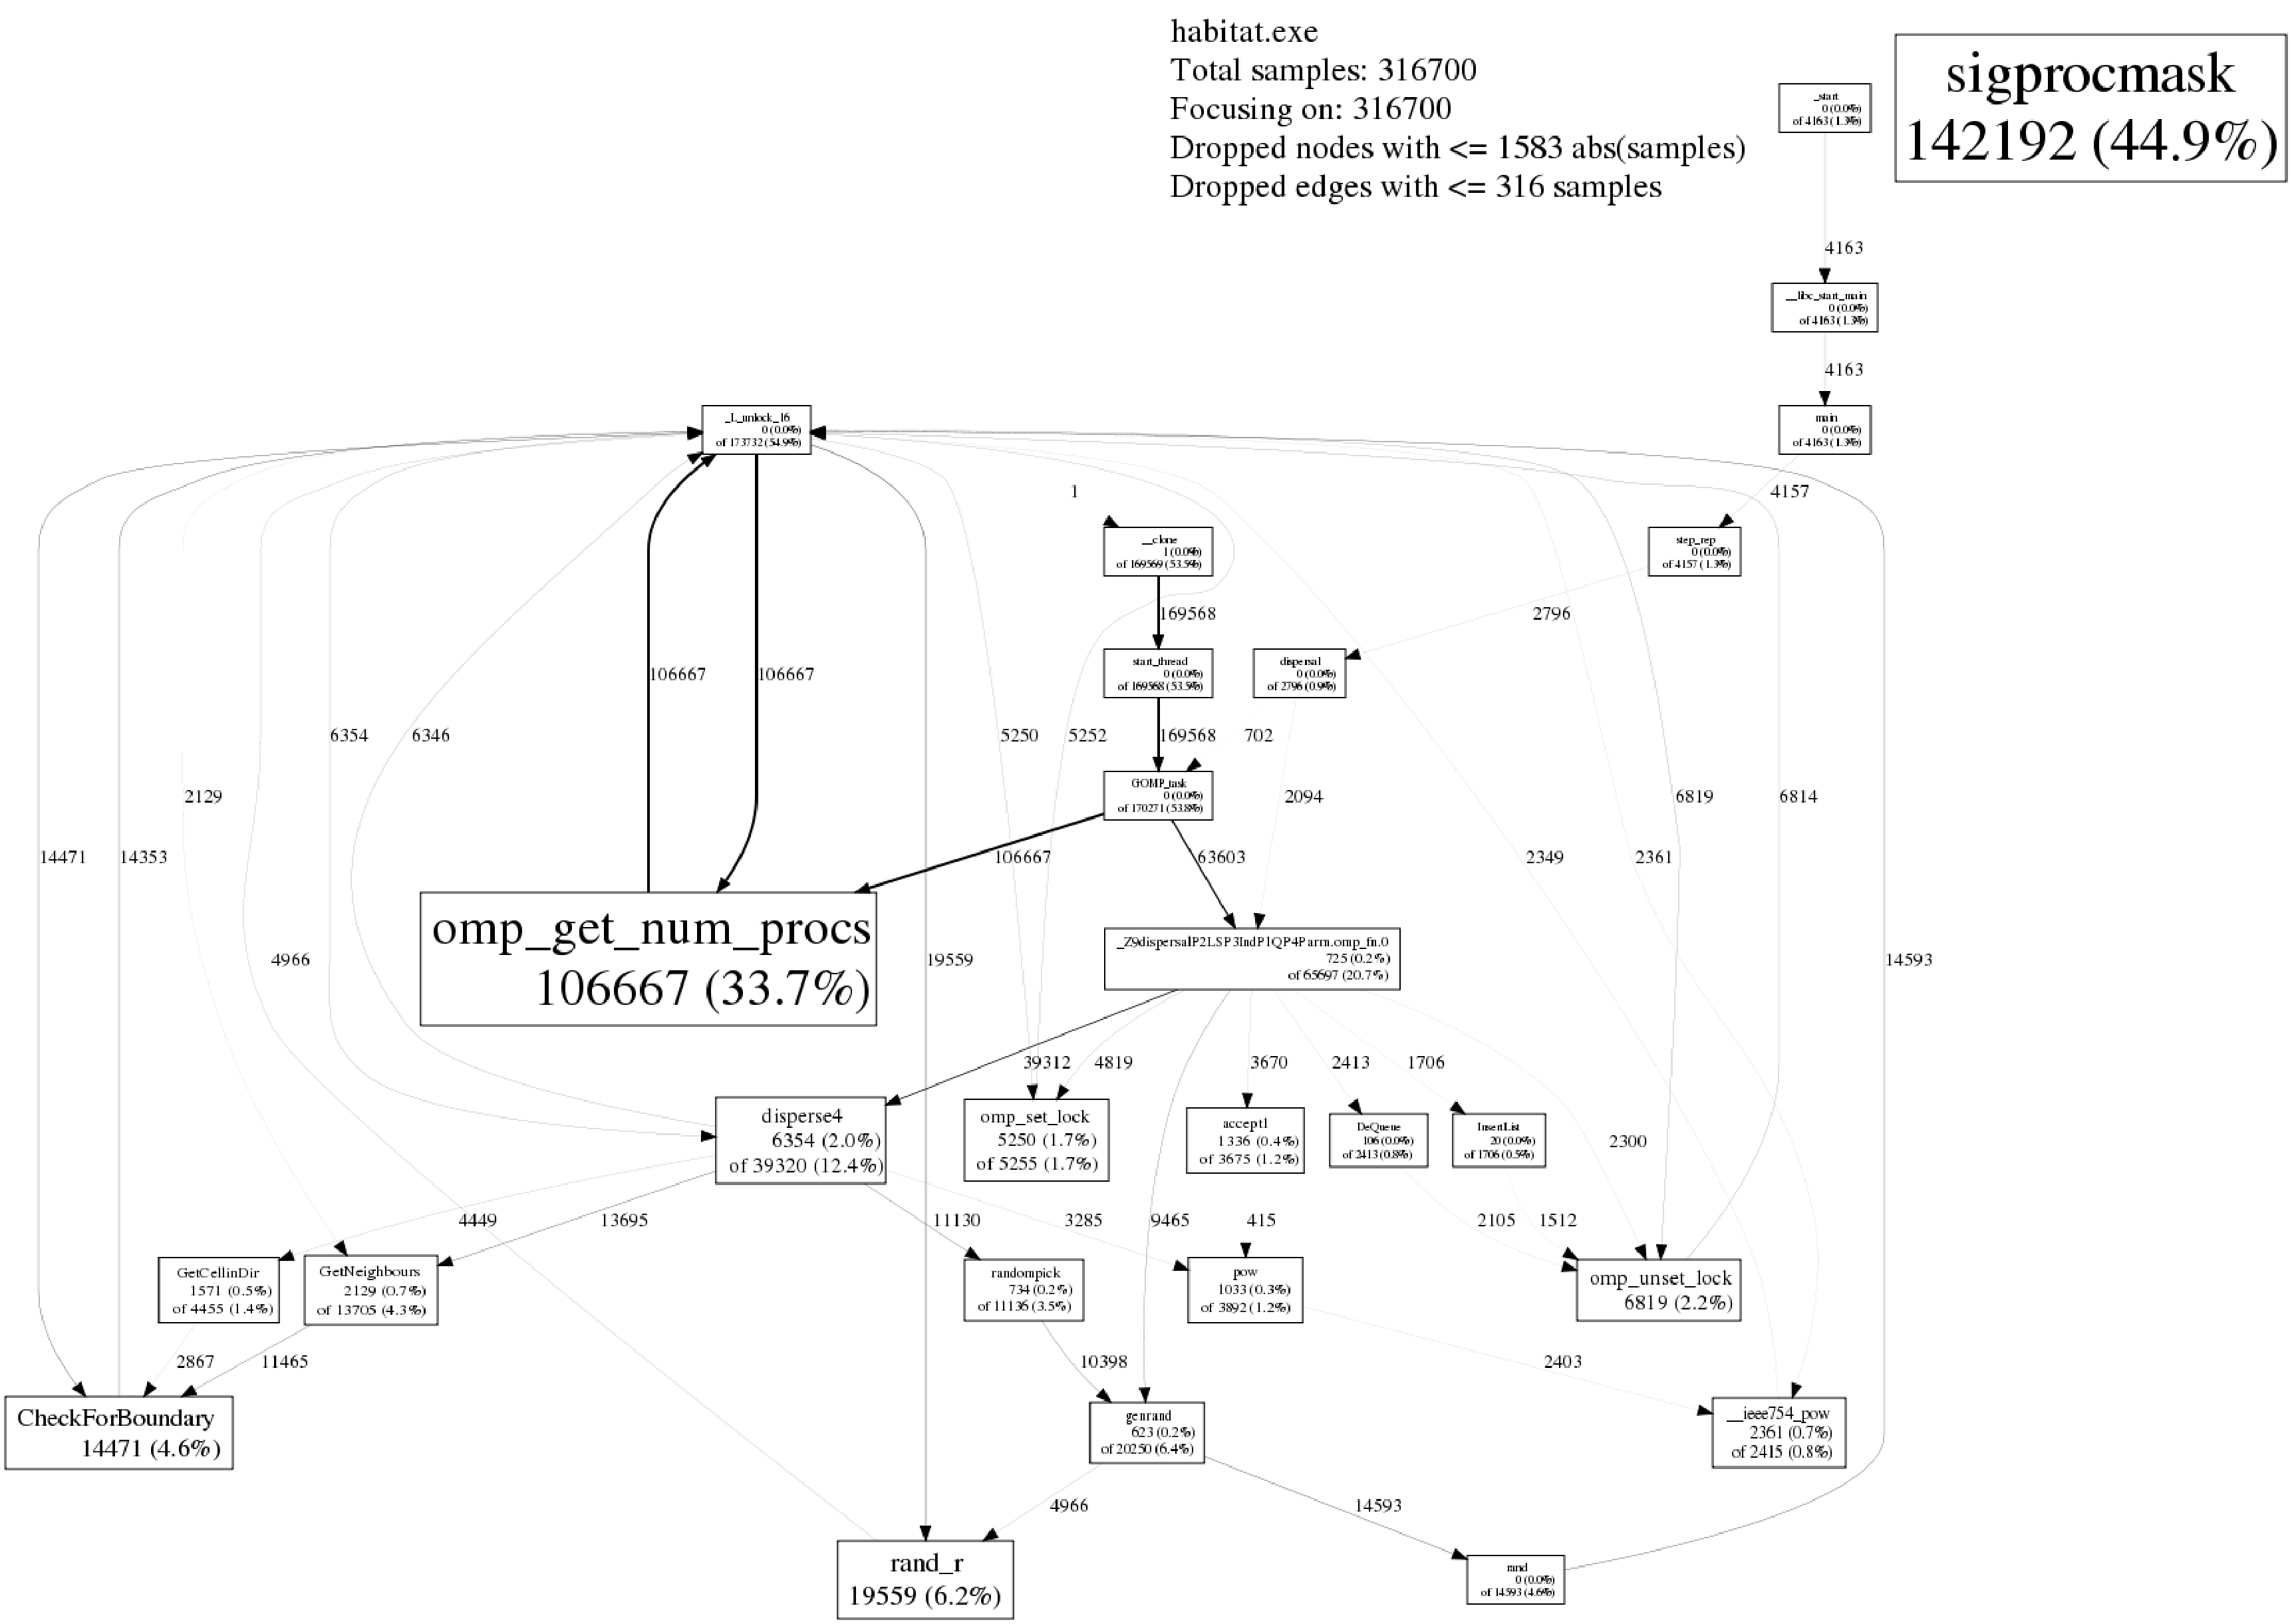
\includegraphics[width=\textwidth]{Include/parallelcall.pdf}
\caption{Call graph for the parallelized habitat simulation} \label{fig:parallelcall}
\end{figure}



\subsection{Replacing random number generator}
The random number generator used in the original application had data races that where detected while running valgrind's helgrind tool.  In order to solve the data races, we replaced the random number generator with a thread safe system provided random generator, \texttt{rand\_r}.  This required adding some saved stated for each thread but provides a thread safe random number generator.  


\section{Evaluation}

In order to evaluate the habitat parallelization, we created input parameters that would span possible parameters used by researchers in the simulation.  The application has two main parameters, the landscape size and the number of starting agents.  Since we parallelized the execution of agents, we expect that the application will scale well with the number of agents.  Also, a larger landscape can handle more agents.  We created input parameter files that included different landscape dimensions and starting agents, as shown in Table \ref{tab:parameters}.

\begin{table}[ht]
\centering
\begin{tabular}{ c | c }
\textbf{Dimensions} & \textbf{Starting Agents} \\ 
\hline \hline
129 x 129 & 300 \\
129 x 129 & 800 \\
200 x 200 & 5000 \\
500 x 500 & 800 \\
500 x 500 & 50000 \\
1024 x 1024 & 1000
\end{tabular}
\caption{Input parameters} \label{tab:parameters}
\end{table}

The habitat executable opens the files \texttt{habitat.in} and \texttt{makeland.in} when it begins execution.  \texttt{habitat.in} contains both the dimensions of the landscape and the number of starting agents.  \texttt{makeland.in} only includes the dimensions of the landscape.

Evaluation jobs where submitted to Tusker with the submission script shown in Listing \ref{lst:submissionfile}.

\begin{figure}[ht]

\lstinputlisting[language=bash,title=pbs.sh,caption={Submission file used for evaluation},label={lst:submissionfile}]{Include/pbs.sh}
\end{figure}

As you can see from the submit script in Listing \ref{lst:submissionfile}, the habitat runs execute in isolation.  First it creates a temporary directory and copies the input files and habitat executable into the temporary directory.  Next it starts the execution and times it.  The stderr of the job includes the job run time.  For the purposes of timing, we use the \texttt{real} time output.

The parameters in Table \ref{tab:parameters} where executed at 7 different core counts: 1, 2, 4, 8, 16, 32, 48.  At each core count, we ran 30 identical jobs to get a good sampling.  For analysis, we averaged the 30 runs at each parameter and core count.  Therefore there where over $7 * 6 * 30 = 1260$ runs.  There where also several re-runs, and a previous set of runs before replacing the random number generator, totaling over 2100 runs of the habitat simulation.

\subsection{Results}

The first set of results are runtimes for one of the runs.

\begin{table}[ht]
\centering
\begin{tabular}{ r | r }
\textbf{Cores} & \textbf{Runtime (m)} \\
\hline \hline
1 & 186.81\\
2 & 142.89\\
4 & 85.59\\
8 & 61.23\\
16 & 37.11\\
32 & 29.49\\
48 & 26.16\\
\end{tabular}
\caption{Runtimes for 1024 x 1024 and 1000 starting agents} \label{tab:runtimes}
\end{table}

1024 x 1024 is a very large landscape for Drew.  He is unable to run a landscape this large on his own machine due to the memory requirements.

\begin{figure}[ht]
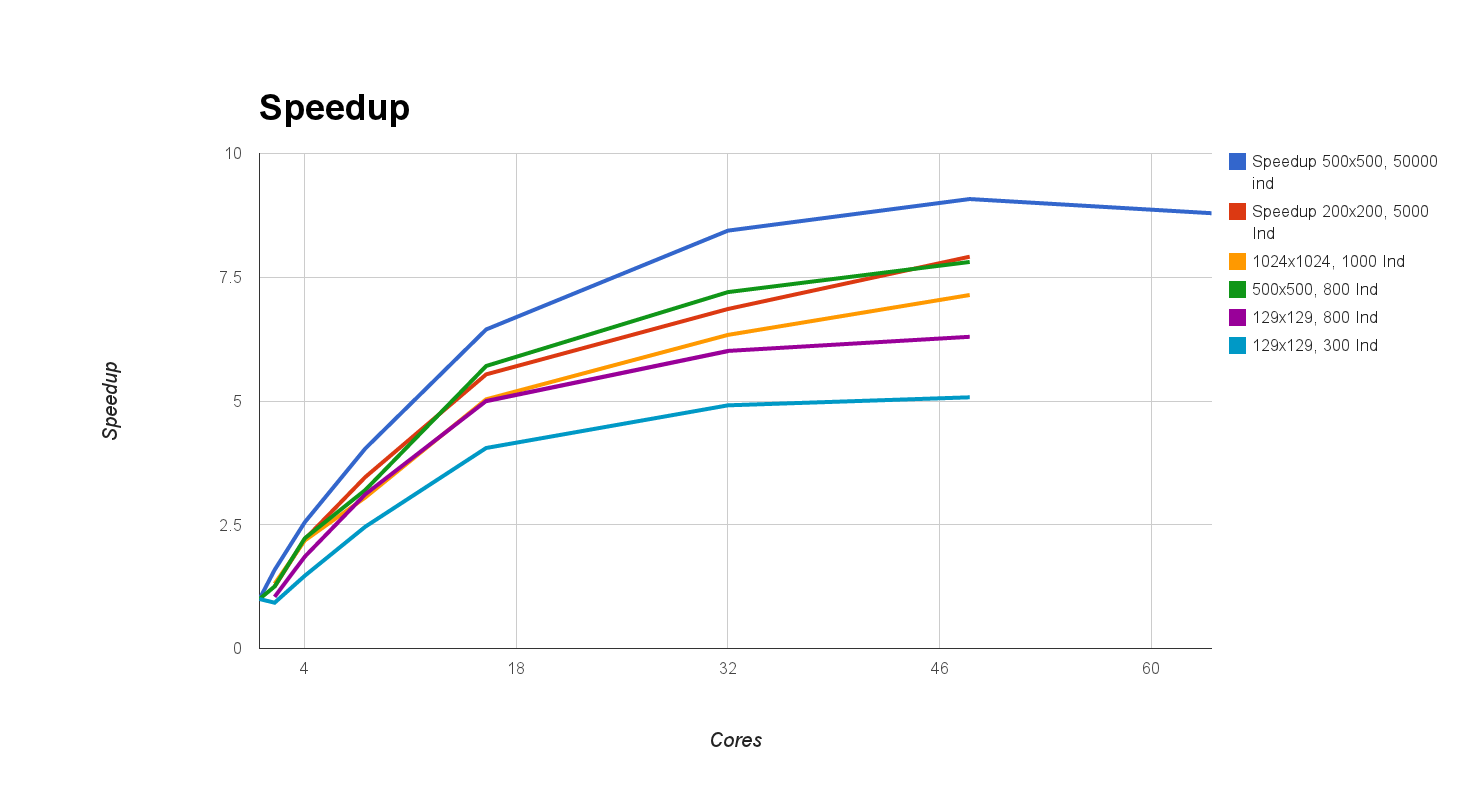
\includegraphics[width=\textwidth]{Include/SpeedupRuns.png}
\caption{Speedup for all Runs} \label{fig:speedup}
\end{figure}


Speedup is shown in Figure \ref{fig:speedup}.  The speedup plateaus for all runs around 32 or 48 cores.  The speedup is limited by the serial portion of the application, which is further described later.  The largest speedup is at the 500x500, with 50000 starting agents.  The large speedup is caused by a very large number of agents, which our parallelization is optimized for.  The speedup peaks at ~9 at 48 cores.

Next we look at efficiency of, shown in Figure \ref{fig:efficiency}.  The efficiency also drops off significantly as the core count increases.

\begin{figure}[ht]
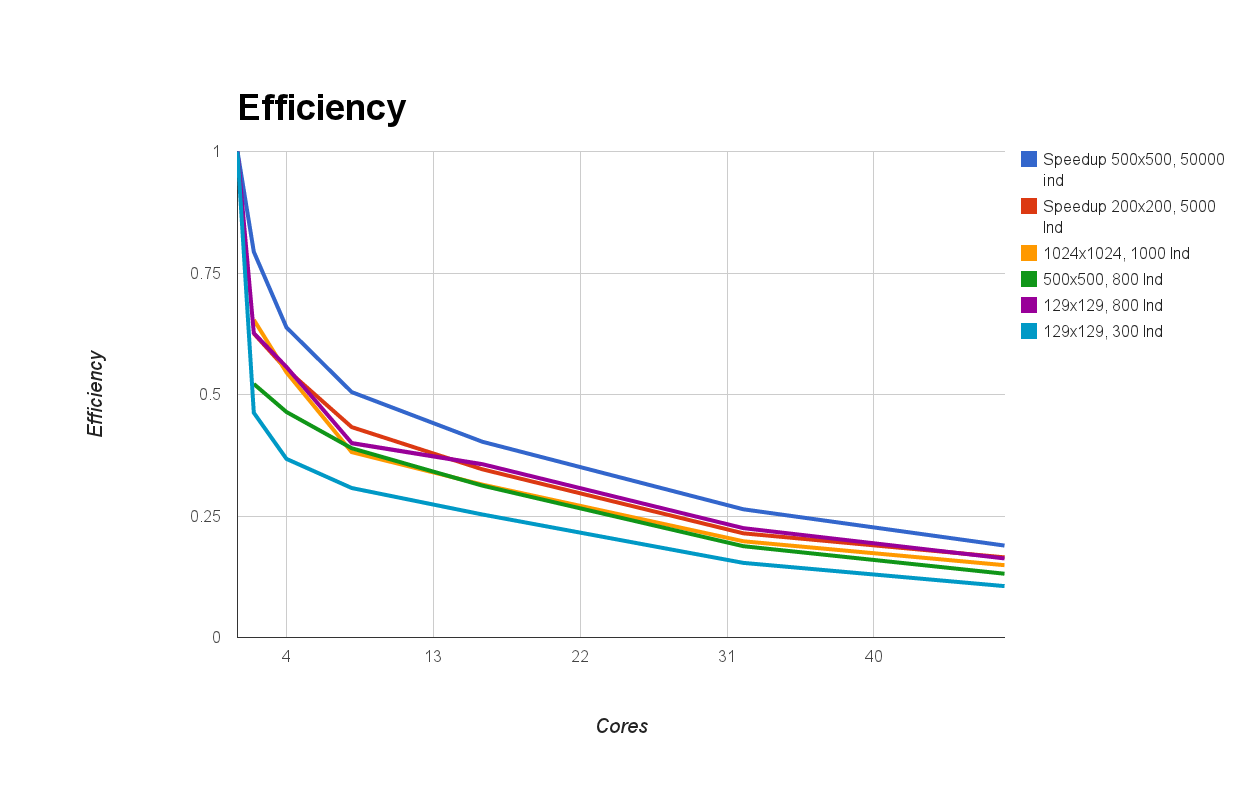
\includegraphics[width=\textwidth]{Include/Efficiency.png}
\caption{Efficiency for all Runs} \label{fig:efficiency}
\end{figure}


Both the efficiency and speedup graphs show that application only scales well to around 32 cores.  To verify that this matches with the expected scalability of the application, we have to first look at the call graph.  The original call graph is shown in Figure \ref{fig:originalcall}.


As you can see in Figure \ref{fig:originalcall}, The parallelized function is \texttt{dispersal}, which callee's takes about 79.0\% of the execution time.  Putting 79\% into Amdahl's law, we can compare the theorized speedup with the actual.  The comparison is shown in Figure \ref{fig:amdahls}.  As you can see, the expected and the actual speedups match nearly in the shape and magnitude.  

\begin{figure}[ht]
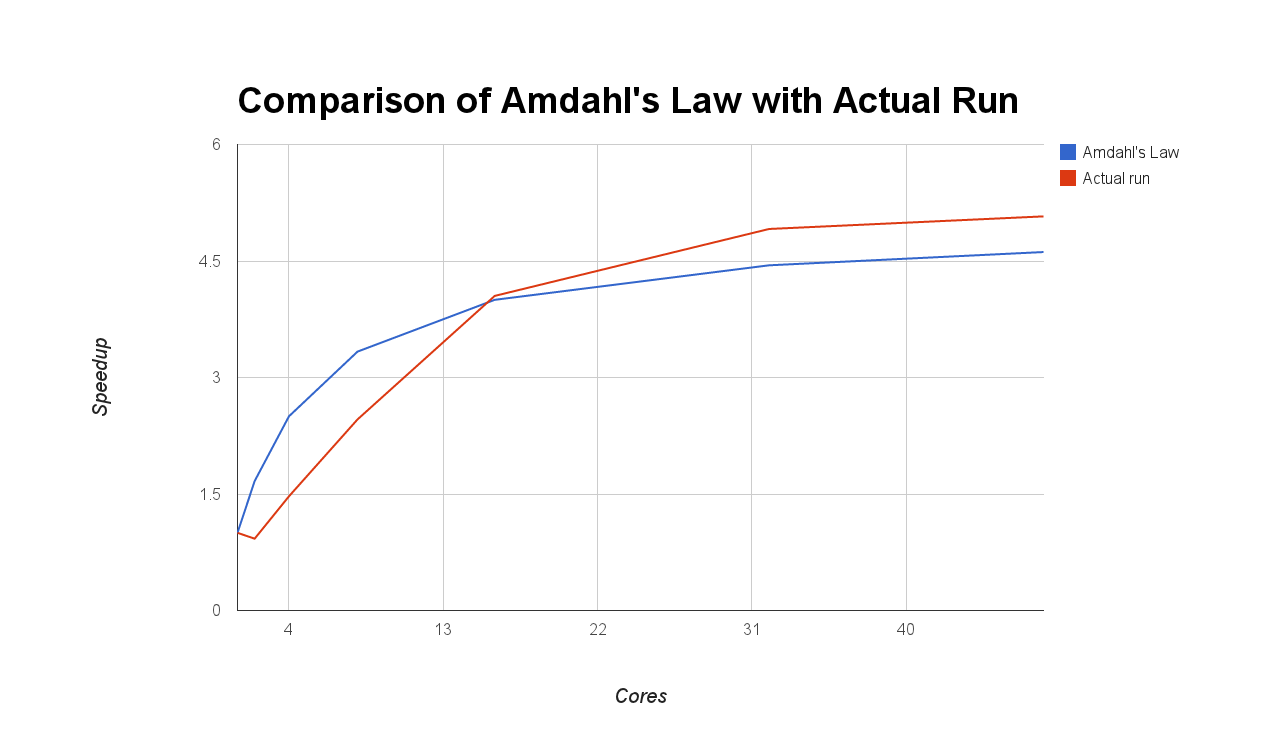
\includegraphics[width=\textwidth]{Include/amdahls.png}
\caption{Comparison of Amdahl's theorized speedup at 79\%} \label{fig:amdahls}
\end{figure}

The parallel call graph is shown in Figure \ref{fig:parallelcall}.  You can see that \texttt{omp\_get\_num\_procs} function is taking a large amount of the processing time.  We could not determine why it is taking so much time, but you can see that it is being called by the OpenMP lock and unlock functions.  We suspect that the google tool that we used to profile is not able to capture calls to the low level kernel locking function.


\subsection{Verification}
For verification, we sent results for our runs to Drew.  He verified the output and generated 2 graphs, shown in Figure \ref{fig:drewgraphs}.  Drew verified that the output appeared accurate.

\begin{figure}[ht]
\centering
\subfloat[Landscape quality] {
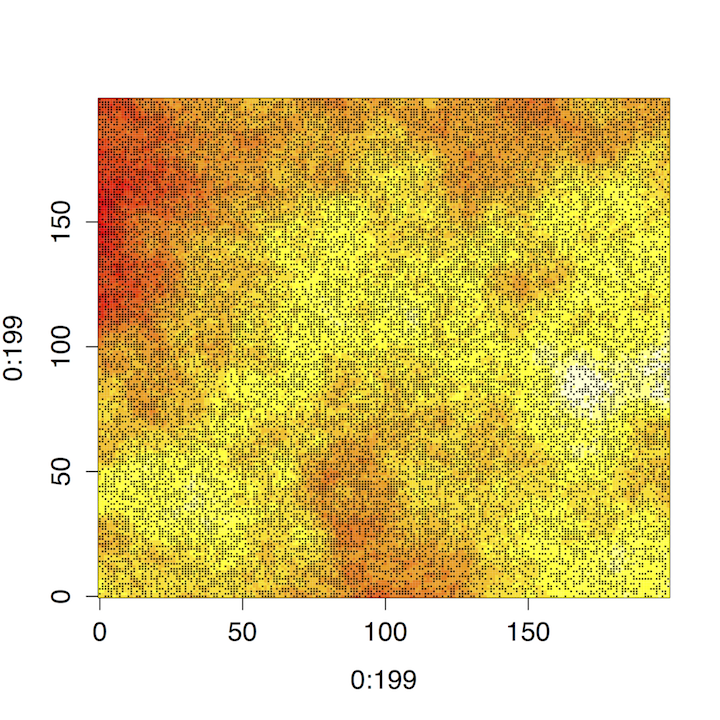
\includegraphics[width=.45\textwidth]{Include/Rplot.png}
}
\subfloat[Agents in the landscape] {
\includegraphics[width=.45\textwidth]{Include/Rplot01.pdf}
}
\caption{Figures made by Drew from the output of a parallel run} \label{fig:drewgraphs}
\end{figure}



\section{Conclusions}
In this project, we parallelized a multi-agent habitat simulation.  We did this by using profiling tools to detect optimal parallelizable sections, and OpenMP to parallelize loops inside the code.  Further, we replaced the random number generator in the simulation with a thread-safe version provided by the system.

We exhaustively evaluated our implementation by running the simulation over a large number of parameters and core counts to determine the speedup of the simulation with our parallelization.  We found that our improvements lead to a speed up of ~9 for large landscapes.  We suspect that larger speedups will be obtained from even larger landscapes and more agents.

We provided the source of our modifications and the scheduler submit files to Drew Tyre on the github page, available at \url{https://github.com/djw8605/habitat}.

\end{document}